Un condensateur de capacité $C = \qty{\v{C}}{\micro\farad}$, initialement déchargé, est branché en série avec une résistance $R = \qty{\v{R}}{\kilo\ohm}$, un interrupteur et une pile idéale de force électromotrice $\mathcal{E} = \qty{\v{eps}}{V}$. On ferme l'interrupteur à $t = 0$.

\begin{center}
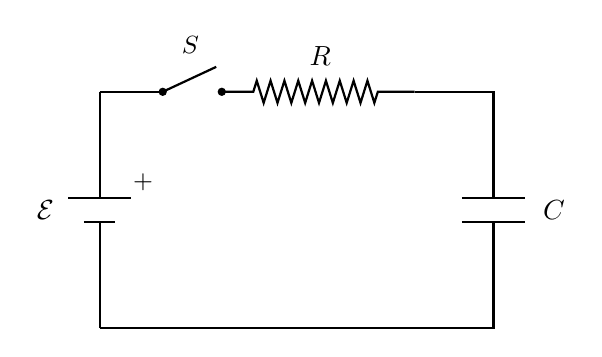
\begin{tikzpicture}[thick, res/.style={decorate,decoration={zigzag,segment length=5pt,amplitude=4pt,pre length=0.4cm,post length=0.4cm}}]
    \draw (0,0) -- (0,1.35);
    \draw (-0.2,1.35) -- (0.2,1.35);
    \draw (-0.4,1.65) -- (0.4,1.65);
    \draw (0,1.65) -- (0,3);
    \node[left] at (-0.45,1.5) {$\mathcal{E}$};
    \node at (0.55,1.85) {\small$+$};
    \draw (0,3) -- (0.8,3);
    \fill (0.8,3) circle (1.5pt);
    \draw (0.8,3) -- ++(25:0.75);
    \fill (1.55,3) circle (1.5pt);
    \node[above] at (1.15,3.35) {\small$S$};
    \draw[res] (1.55,3) -- (4,3);
    \node[above] at (2.8,3.2) {$R$};
    \draw (4,3) -- (5,3) -- (5,1.65);
    \draw (4.6,1.65) -- (5.4,1.65);
    \draw (4.6,1.35) -- (5.4,1.35);
    \node[right] at (5.5,1.5) {$C$};
    \draw (5,1.35) -- (5,0) -- (0,0);
\end{tikzpicture}
\end{center}

\begin{enumerate}[label=\alph*)]
    \item Déterminez la constante de temps du circuit.
    \item Déterminez la charge du condensateur à $t = \qty{\v{t}}{ms}$.
    \item Déterminez le courant dans le circuit à ce même instant.
    \item Combien de temps après la fermeture de l'interrupteur la charge atteint-elle \qty{90}{\percent} de sa valeur finale ?
\end{enumerate}
